This section describes the experiments performed as proof of concept to the algorithm.
The Rhone prototype is implemented in Java.
It includes 15 java classes in which 14 of them model the basic concepts 
(\textit{query}, \textit{abstract services}, \textit{concrete services}, etc), 
and 1 responsible to implement the core of the algorithm. 

Currently, our approach runs in a controlled environment. 
Different experiments were produced to analyze the algorithm's behavior.
We will present two experiments: \textit{experiment 1} and \textit{experiment 2}.
The service registry used has 100 concrete services. 
In each experiment, there are a set of tests in which the number of concrete 
services varies from 5 until to reach 100.

\begin{figure}[!h]
\centering
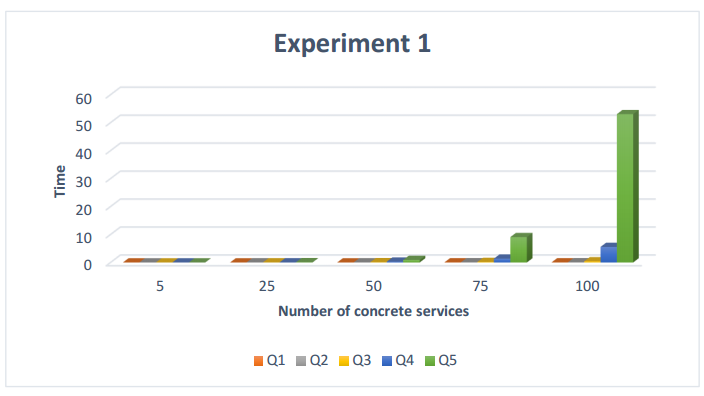
\includegraphics[scale=0.4]{exp1.png}
\caption{Query rewriting evaluation.}\label{fig01}
\end{figure} 

In the \textit{experiment 1}(figure~\ref{fig01}), there are five different queries that differ on
the quantity of abstract services (increasing from 2 to 6). Analyzing the first
experiment, it is easily to identify that the algorithm shares the same problem
as existing query rewriting approaches using views: increasing the
processing time when the size of the query and the number of concrete services increase.

%\begin{figure}[!h]
%\centering
%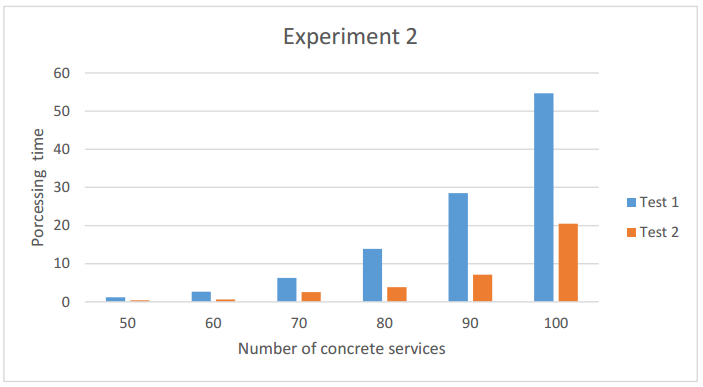
\includegraphics[scale=0.4]{exp2.png}
%\caption{Query rewriting evaluation.}\label{fig02}
%\end{figure} 

The \textit{experiment 2} (figure~\ref{fig:fig02}) presents the results while testing the algorithm in the presence of user preferences and services' quality aspects extracted from SLAs.  The difference between \textit{Test 1} and \textit{Test 2} concerns the way services are selected and the query is rewritten. Once \textit{Test 1} do not consider quality measures as any other existing query rewriting approach, \textit{Test 2} uses the user preferences statements and services' quality aspects to guide the service selection and query rewriting.
Both include queries with six abstract services and quality requirements concerning availability, response time, price per call and integration cost (total cost). The figure~\ref{fig:fig02} shows our results. 

%\begin{figure}[!h]
%\centering
%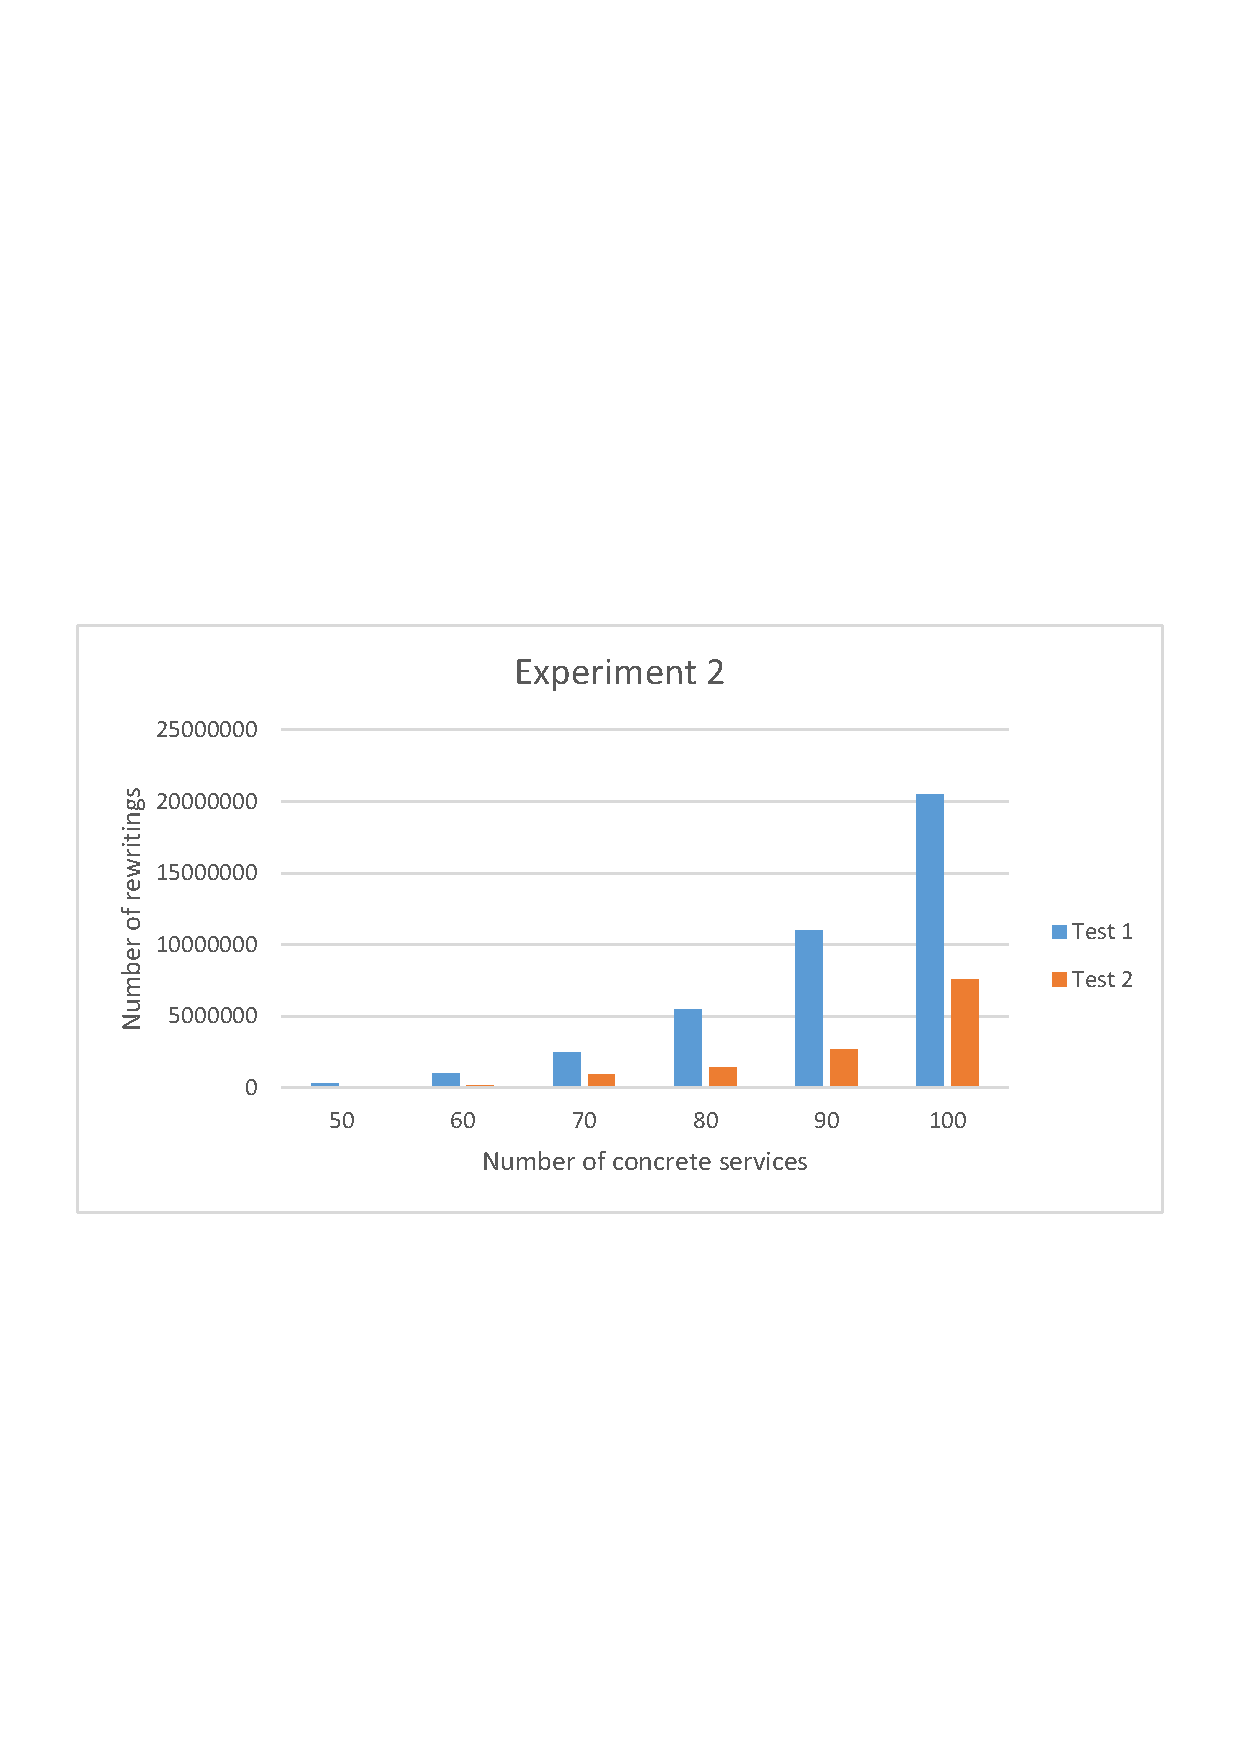
\includegraphics[scale=0.4]{exp3.png}
%\caption{Query rewriting evaluation.}\label{fig03}
%\end{figure} 


\begin{figure}%
\centering
\parbox{2.2in}{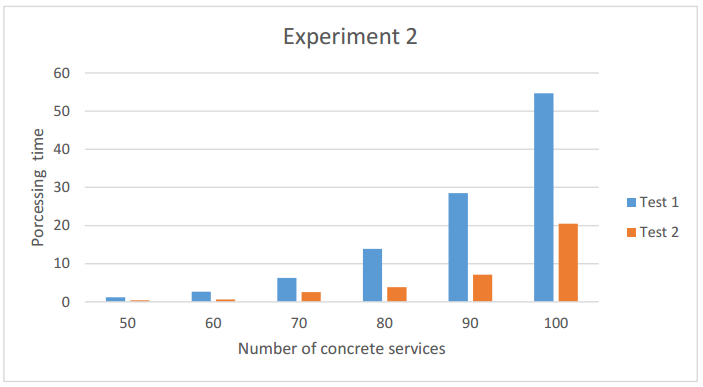
\includegraphics[scale=0.30]{exp2.png}}% 
\qquad
\begin{minipage}{2in}%
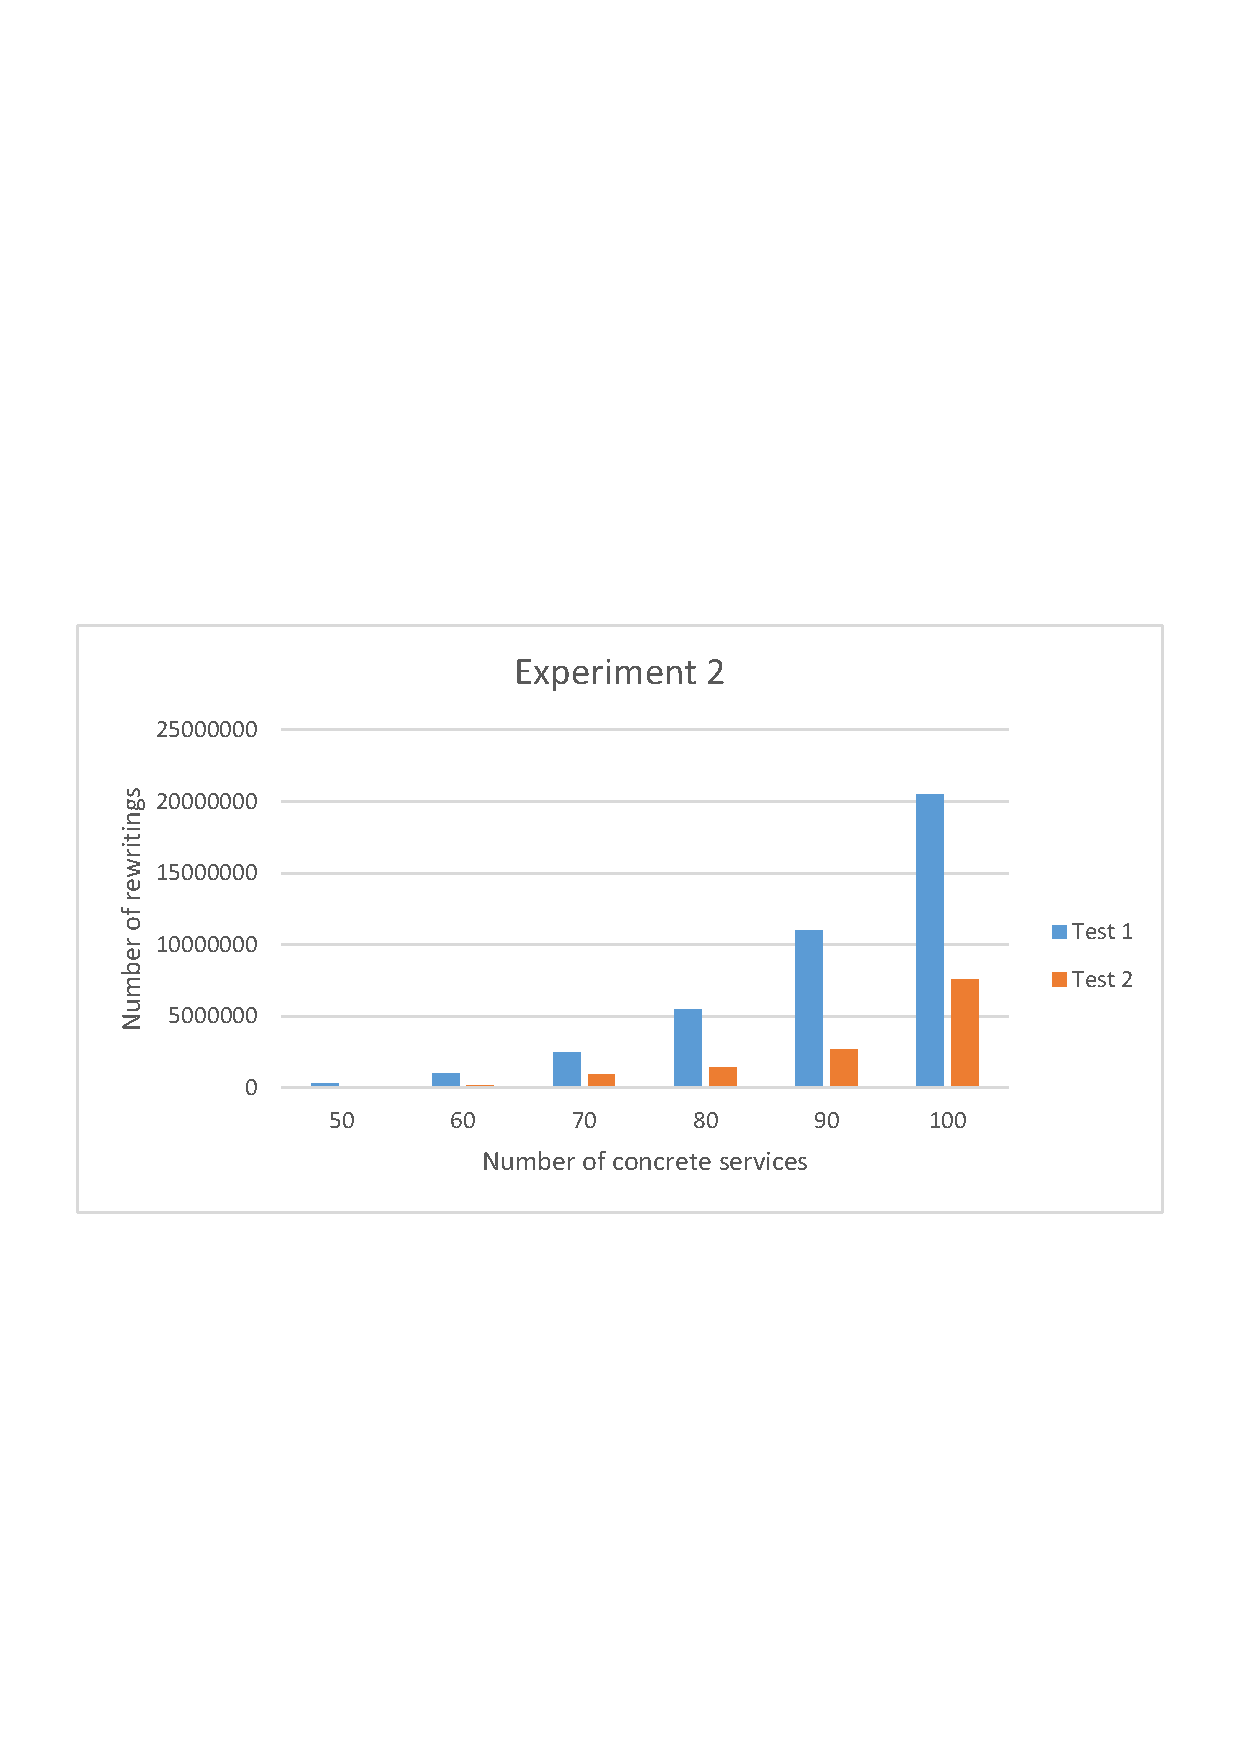
\includegraphics[scale=0.30]{exp3.png}
\end{minipage}%
\caption{Results concerning processing time (left-side) and rewritings number (right-side).}%
\label{fig:fig02}%
\end{figure}

The results while considering user preferences and SLAs are promisingly.  
%The \textit{Rhone} presents a better performance, decreasing the processing time and 
%the total number of rewritings produced.  
%Reducing rewriting number allow to go straightforward to the rewriting solutions that are satisfactory avoiding any further backtrack.
The \textit{Rhone} increases performance reducing rewriting number (around 50 percent) which allows to go straightforward to the rewriting solutions that are satisfactory avoiding any further backtrack and thus reducing successful integration time. Moreover, once the services selection and service composition (rewritings) process are fully guided by the user requirements and SLA, the algorithm avoid producing and executing composition that are not interest for the user. In this sense, the reduces the integration economic cost while delivering the expected results.